\section{System Overview}
\label{sec:architecture}

FHEStore connects persistent application data to an external FHE evaluator through two storage-side paths: an input path for preprocessing, encoding, and encryption, and a return path for decryption, decoding, and result write-back. The host coordinates these paths through operator programs and relays ciphertext batches to and from the remote service.

\subsection{System Organization}
\label{subsec:system-organization}

Figure~\ref{fig:pipeline} shows the three components of FHEStore's execution environment: an FPGA-based computational storage device (CSD), a host, and a remote FHE service. The CSD combines persistent storage, device-local buffers, a device runtime, and FPGA operators. Its input path supplies stored data to optional preprocessing and then to an integrated encoding and encryption operator. Its return path supplies result ciphertexts to an integrated decryption and decoding operator and passes recovered application values to write-back.

\begin{figure*}[t]
  \centering
  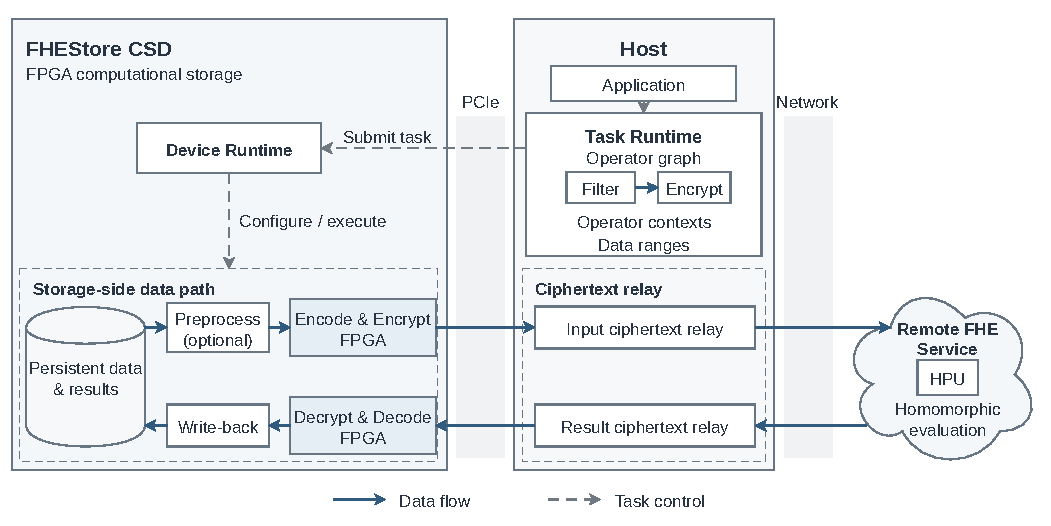
\includegraphics[width=\textwidth]{figures/fhestore-overview-v3/fhestore-overview.pdf}
  \caption{FHEStore system organization. PCIe carries task control and ciphertext handoffs between the host and CSD; the network carries ciphertexts between the host relay and remote FHE service. Solid arrows denote logical data flow, and dashed arrows denote control flow. The storage-side data path is a functional boundary; record write-back may involve host-assisted read--modify--write.}
  \Description{The computational storage device contains storage, a device runtime, optional preprocessing, FPGA encoding and encryption, FPGA decryption and decoding, and functional write-back. The host contains an application, a task runtime describing an operator graph, contexts, and data ranges, and input and result ciphertext relays. The host submits tasks and exchanges ciphertexts with the device over PCIe. It relays input ciphertexts to a remote HPU service over the network and returns result ciphertexts to the device for recovery and write-back.}
  \label{fig:pipeline}
\end{figure*}

The host has two roles. Its task runtime translates application requests into operator graphs, per-operator contexts, and data ranges for device execution. Its ciphertext relay retrieves generated ciphertexts from the CSD and forwards them to the remote service, then stages returned ciphertexts for the CSD's decryption path. PCIe connects the host and CSD and carries both task control and ciphertext transfers. The host communicates with the remote service over a network; the prototype uses TCP. The remote HPU performs homomorphic evaluation on the supplied ciphertexts.

The host and CSD belong to the data owner's trusted processing domain because preprocessing, decryption, and record merging access plaintext. The host provisions the local cryptographic operators with secret-key material through their contexts. The remote service is provisioned with the corresponding evaluation keys and operates on ciphertexts.

\subsection{Application Task Model}
\label{subsec:application-task}

An application specifies a task $T=(D,Q,E,O)$, comprising source data $D$, preprocessing $Q$, cryptographic configuration $E$, and a downstream action $O$. Table~\ref{tab:task-contract} summarizes these fields. For record-oriented inputs, $D$ identifies a storage namespace and block range together with a schema specifying record width, field types, and byte offsets. The selective prototype evaluates predicates over integer fields and projects an unsigned 8-bit field for encryption. Direct encryption uses the supplied application values and bypasses preprocessing.

\begin{table}[ht]
  \caption{Application task fields and their roles in FHEStore.}
  \label{tab:task-contract}
  \centering
  \small
  \setlength{\tabcolsep}{3pt}
  \begin{tabular}{@{}p{0.24\columnwidth}p{0.70\columnwidth}@{}}
    \toprule
    Field & Task declaration \\
    \midrule
    Source $D$ & Storage namespace and range, record count, and schema. \\
    Preprocessing $Q$ & Selection predicate and projected field. \\
    Crypto $E$ & Encoding and cryptographic parameters, with a local key reference. \\
    Action $O$ & Ciphertext delivery, or a remote operation and result destination. \\
    \bottomrule
  \end{tabular}
\end{table}

For records $r_0,\ldots,r_{N-1}$, let $P_Q$ be the selection predicate and $\pi_Q$ the projection. The ordered index sequence $\mathcal{I}_Q=(i_0,\ldots,i_{M-1})$ contains the records satisfying $P_Q$, in source-record order. The input path produces
\begin{equation}
  c_j = \operatorname{Enc}_{E}\!\left(
    \operatorname{Encode}_{E}\!\left(\pi_Q(r_{i_j})\right)
  \right),\quad 0\leq j<M.
  \label{eq:task-ciphertexts}
\end{equation}
Here, $c_j$ denotes the ciphertext bundle representing one application value; its constituent LWE ciphertexts follow the encoding specified by $E$. The host retains $\mathcal{I}_Q$ alongside the ciphertext sequence. In the elementwise update workflow, the $j$th returned value is associated with record $i_j$, allowing the result to be placed into the selected field of that record.

Task semantics are separate from execution settings. A runtime profile selects device endpoints, batch size, and transfer granularity. The host divides the source into block-aligned batches and attaches a record-base offset to each batch, preserving global record identities across the task. The same task can stop after ciphertext generation or continue through remote evaluation and result write-back, according to $O$.

\subsection{Operator Graphs and Device Execution}
\label{subsec:operator-execution}

The task runtime represents a device execution as an operator program, a set of operator contexts, and a set of input and output memory ranges. The program identifies the operator types and their stream connections. Contexts supply parameters such as record layout, predicates, projected fields, and cryptographic configuration. Memory ranges identify the device buffers and byte extents used by an invocation. Together, these objects connect the task's logical operations to its concrete input and output data.

The host loads and activates the program through the CSD interface and submits an execution request with the contexts and range bindings. The device runtime maps logical operator identifiers to available physical FPGA instances and configures their stream connections and buffer transfers. For selective input preparation, the graph connects the filtering and projection operator directly to encoding and encryption, so projected values flow between the FPGA operators within the CSD. Direct encryption uses a single cryptographic operator. The return path uses a separate decryption program whose input range contains returned ciphertexts and whose output range receives decoded application values.

Selection determines the cryptographic workload and the required output capacity. For each selective batch, device-generated selection metadata supplies the selected count and record indices to the host. The host uses this count and the per-value ciphertext size to bind the generation program's output range. Selection discovery and ciphertext generation operate on the same buffered input image, keeping the count, ciphertext order, and record mapping consistent. A batch with no selected records skips encryption and remote evaluation.

\subsection{Ciphertext Handoff and Result Write-Back}
\label{subsec:ciphertext-handoff}

At the CSD--host handoff, the host uses the device-reported output length and the task's cryptographic configuration to form a network request. Each request carries an identifier, ciphertext-shape metadata, and the ciphertext payload. The prototype checks the response identifier and metadata before supplying the returned batch to the decryption path. Encoding, cryptographic parameters, and ciphertext serialization must agree across input production, remote evaluation, and result recovery.

The host transfers the returned ciphertexts over PCIe into a device-local input buffer and invokes the FPGA decryption and decoding operator. Recovered application values are then written according to the task's destination policy. For contiguous outputs, the device copies the decrypted output buffer to a designated SSD range. For selected-record updates, the host uses the retained index sequence to merge recovered values into record pages and writes the resulting record image to the specified destination. This merge preserves unselected records and the other fields of selected records.

The application distinguishes completion of ciphertext generation, receipt of a remote response, and completion of result write-back. A generation-only task completes when its ciphertext output and record mapping are available. An update task also waits for result recovery and destination I/O. The task interface uses a separate destination range for selected-record updates, and the prototype verifies the written record image by reading it back.
